\section{Tietorakenteen arviointi}\label{tulokset}

Luvussa \ref{mun} esitettiin sisäkkäispistepuun solmujen sisältämien ruudukoiden mahdollistama yksinkertainen kompressiotekniikka ja algoritmeja puun rakentamiseen ja renderöintiin. Luvussa \ref{rakentaminen} mitataan sisäkkäispistepuun rakentamisen, tallentamisen ja läpikäynnin suorituskykyä ja arvioidaan kompression vaikutusta siihen. Luvussa \ref{renderöinti} mitataan pistepilvien renderöintinopeutta eri tekniikoilla. Testikoneessa on Intel i7-8850H -suoritin, 32 gigatavua keskusmuistia, SSD-levy ja Nvidia Quadro P2000 -näytönohjain.  

\subsection{Tietorakenteen rakentaminen ja lataaminen}\label{rakentaminen}

Tietorakenteen rakentamista, tallentamista ja muistiin lataamista arvioitiin kolmella pistepilvellä. \emph{Pannuhuone}-pilvi sisälsi 20 keilausta, jotka veivät 18,7 gigatavua tilaa tallennettuna ascii-formaatissa. Keilauksista muodostettiin puu, jossa oli 546572600 pistettä 528017:ssa solmussa, jotka jakautuivat yhdeksälle tasolle. \emph{Toimisto} sisälsi 8,43 gigatavua pisteitä 21 keilauksesta ja siitä muodostetussa puussa oli 240727221 pistettä 608002:ssa solmussa 11:llä tasolla. \emph{Pumput} oli testattavista pienin, vain 41:n megatavun kokoinen pistepilvi. Siinä oli 5 keilausta, joista rakennetussa puussa oli 1213990 pistettä 4561:ssä solmussa seitsemällä tasolla.  

\begin{table}[h]
    \begin{tabular}{llll}
    \hline
    pisteiden esitysmuoto & tiedoston koko & rakentaminen ja tallentaminen & läpikäynti \\ \hline
    16 tavua       & 8,17 GB             & 2574s = 42min 54s              & 6227ms     \\
    8 tavua        & 4,10 GB             & 1652s = 27min 32s             & 16190ms    \\
    4 tavua        & 2,07 GB             & 1602s = 26min 42s             & 13462ms    \\ \hline
    \end{tabular}
    \caption{Pannuhuone-pilvestä muodostetun oktettipuun rakentaminen ja pisteiden läpikäyminen}
    \label{taulukko:pannuhuone}
\end{table}


\begin{table}[h]
    \begin{tabular}{llll}
    \hline
    pisteiden esitysmuoto & tiedoston koko & rakentaminen ja tallentaminen & läpikäynti \\ \hline
    16 tavua & 3,59GB              & 891s = 14min 51s              & 2763ms     \\
    8 tavua  & 1,83GB              & 724s = 12min 4s               & 8492ms     \\
    4 tavua & 961MB               & 712s = 11min 52s              & 6985ms     \\ \hline
    \end{tabular}
    \caption{Toimisto-pilvestä muodostetun oktettipuun rakentaminen ja pisteiden läpikäyminen}
    \label{taulukko:toimisto}
\end{table}

\begin{table}[h]
    \begin{tabular}{llll}
    \hline
    pisteiden esitysmuoto & tiedoston koko & rakentaminen ja tallentaminen & läpikäynti \\ \hline
    16 tavua       & 18,6MB              & 12s                           & 14ms       \\
    8 tavua      & 9,57MB              & 10s                           & 36ms       \\
    4 tavua      & 4,94MB              & 9s                            & 29ms       \\ \hline
    \end{tabular}
    \caption{Pumput-pilvestä muodostetun oktettipuun rakentaminen ja pisteiden läpikäyminen}
    \label{taulukko:pumput}
\end{table}

Taulukoissa \ref{taulukko:pannuhuone}, \ref{taulukko:toimisto} ja \ref{taulukko:pumput} on mitattu testipilvien rakentamiseen, tallentamiseen ja pisteiden läpikäyntiin kuluva aika käyttäen kolmea luvussa \ref{kompressio} käytettyä pisteiden esitysmuotoa: maailmakoordinaatit ja väri (16 tavua), ruudukon solun indeksi ja väri (8 tavua), sekä solun suhteelliset koordinaatit ja valon heijastumisen intensiteetti (4 tavua). 

Yllätyksettömästi 16:n tavun pistedatan muistiin lataaminen ja läpikäyminen oli huomattavasti nopeampaa kuin kompressoitujen pisteiden. Nelitavuisten pisteiden lataaminen ja kompression purkaminen oli nopeampaa kuin kahdeksantavuisten. Tietorakennetta rakentaessa näyttää siltä, että pistedatan kirjoittaminen levylle vie huomattavan osan suoritusajasta. Tästä syystä on ajansäästön kannalta kannattavaa käyttää laskenta-aikaa pistedatan kompressointiin, jotta kirjoitettavia tavuja olisi vähemmän. 


\subsection{Renderöinti}\label{renderöinti}

Tietorakenteen renderöitiä arvioitaessa käytetään kahta pistepilveä. \emph{Ilmanvaihtohuone} on keilattu Elomatic Oy:n Jyväskylän toimiston ilmanvaihdon konehuoneesta ja siinä on 13 keilausta, joista muodostetussa puussa on 506366789 pistettä 267641 solmussa kahdeksassa tasossa. \emph{wroksite}-pilvi on Leica Geosystemsin testidataa, joka sisältää 7 keilausta, joiden 53881180 pistettä jakautuu 543105 solmuun yhdeksälle puun tasolle. 

\begin{figure}[h]
    \centering
    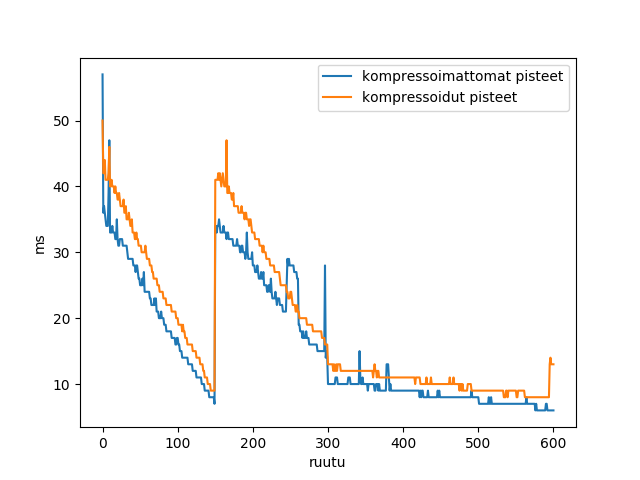
\includegraphics[width=0.9\textwidth]{tuloksia/worksite_compressed_vs_uncompressed.png}
    \caption{Worksite-pilven kahden miljoonan pisteen renderöintiin vaadittu aika millisekunteina käyttäen kompressoimattomia 16:n tavun pisteitä ja kahdeksaan tavuun kompressoituja pisteitä.}
    \label{ws_compr}
\end{figure}

Arvioidaan ensin luvussa \ref{kompressio} esitellyn kompression vaikutusta pistepilven renderöintiaikaan. Kuvassa \ref{ws_compr} on esitetty kaavio kahden miljoonan pisteen renderöinnin vaatimasta ajasta kamera-ajon jokaisella ruudunpäivityksellä. Sininen viiva kuvaa renderöintiaikaa kompressoimattomilla pisteillä ja oranssi viiva värit säilyttävällä kompressiolla. Renderöinnissä on käytetty luvussa \ref{render} esiteltyä puskurivirta-algoritmia. 

Kamera-ajo alkaa maiseman reunalta ja kulkee työmaan ohi lähestyen sen reunaa siten, että näkyvissä olevien puun solmujen määrä laskee tasaisesti. Tämä näkyy myös kuvassa \ref{ws_compr} ruudun renderöintiajan laskiessa. Näkymäkarton sisällä olevien solmujen määrä kasvaa äkkinäisesti noin 150:nnen ruudun kohdalla, jolloin kamera kääntyy niin, että koko pilvi on näkyvissä. Lopuksi kamera lähestyy vastakkaista seinää ja näkyvissä olevien solmujen määrä laskee. 

Kuvaajasta huomataan, että kompressoimattomien 16-tavuisten pisteiden renderöinti on jonkin verran nopeampaa kuin kompressoitujen kahdeksantavuisten pisteiden. Eron selittää kompression avaamiseen vaadittu laskenta. Jokaisesta kompressoidusta pisteestä etsitään kompressoidun pisteen indeksiä vastaava ruudukon solu ja lasketaan sen keskipiste. Renderöintiajan ero on kuitenkin pieni ja voidaan katsoa, että miltei puolittunut tallennustilan tarve oikeuttaa pistedatan kompression.

\begin{figure}[h] 
    \centering
    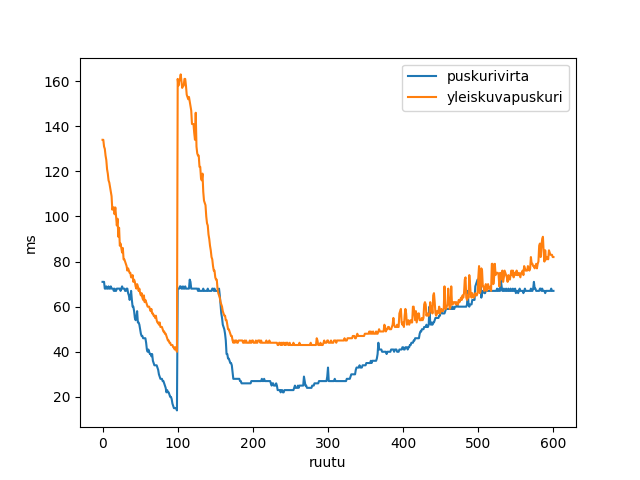
\includegraphics[width=0.9\textwidth]{tuloksia/ilmanvaihtohuone_ms_per_frame.png}
    \caption{Ilmanvaihtohuone: kahden miljoonan pisteen renderöintiin vaadittu aika millisekunteina kahdella eri renderöintialgoritmilla.}
    \label{iv_ms}
\end{figure}

Luvussa \ref{render} esiteltiin puskurivirran lisäksi yleiskuvapuskuria käyttävä algortimi, joka pitää osaa pistepilvestä näytönohjaimen muistissa. Kuvassa \ref{iv_ms} on mitattu kahden miljoonan pisteen renderöintiaikaa ilmanvaihtohuone-pilvessä. Sininen viiva kuvaa renderöintiaikaa käytettäessä pelkkää puskurivirtaa ja oranssin viivan kuvaamassa mittauksessa on ensin renderöity yleiskuvapuskuri, minkä jälkeen jäljelle jäävät puun solmut on järjestetty kuvaruudulle projisoidun koon mukaan ja renderöity puskurivirralla. Yleiskuvapuskurissa on puun neljä ensimmäistä tasoa, joissa on yhteensä 286 solmua ja niissä 723834 pistettä.

Ilmanvaihtohuoneen kamera-ajo alkaa huoneen reunalta kameran osoittaessa vastakkaiselle seinälle. Kamera liikkuu kohti vastakkaista seinää, jolloin renderöitävien solmujen määrä vähenee. Kameran saavutettua vastakkaisen seinän noin sadan ruudun jälkeen se kääntyy ympäri osoittamaan huoneen poikki. Näkyvissä olevien solmujen äkkinäinen kasvaminen näkyy jyrkkänä piikkinä kuvassa \ref{iv_ms}. Tämän jälkeen kamera lähestyy taas seinää ja renderöintiaika kasvaa. Lopuksi kamera peruuttaa pois päin seinästä ja näkyvillä olevien solmujen kasvava määrä pitkittää ruutujen renderöintiä.

\begin{figure}[h]
    \centering
    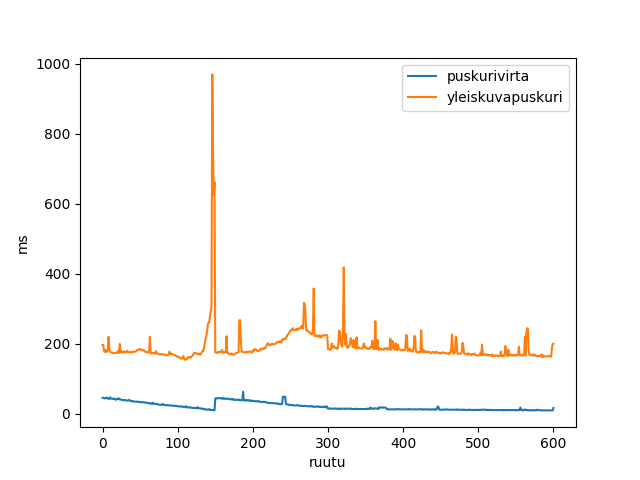
\includegraphics[width=0.9\textwidth]{tuloksia/worksite_ms_per_frame.png}
    \caption{Worksite-pilven kahden miljoonan pisteen renderöintiin vaadittu aika millisekunteina kahdella eri renderöintialgoritmilla}
    \label{ws_ms}
\end{figure}

Kuvassa \ref{ws_ms} on tehty vastaavat mittaukset worksite-pilvelle. Oranssin viivan kuvaamassa renderöintitavassa on yleiskuvapuskurissa puun viisi ylintä kerrosta, 1862 solmua ja 481663 pistettä.

\begin{figure}
    \subfloat[]{
        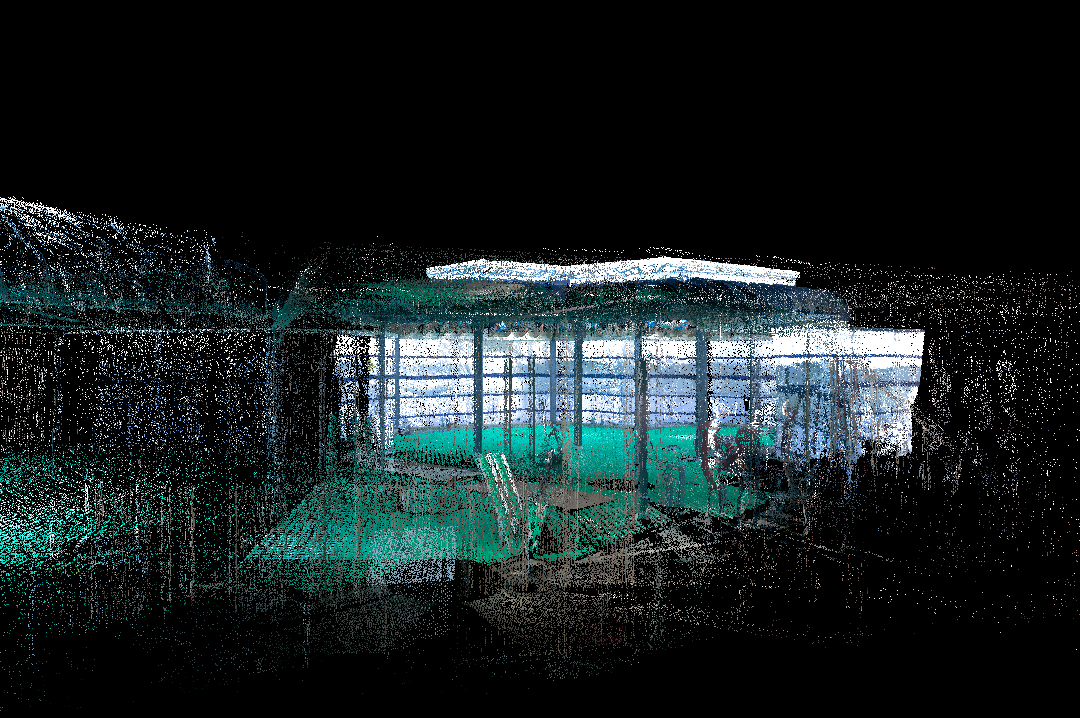
\includegraphics[width=.5\linewidth]{tuloksia/worksite_2M/worksite_stream.png}
    }
    \subfloat[]{
        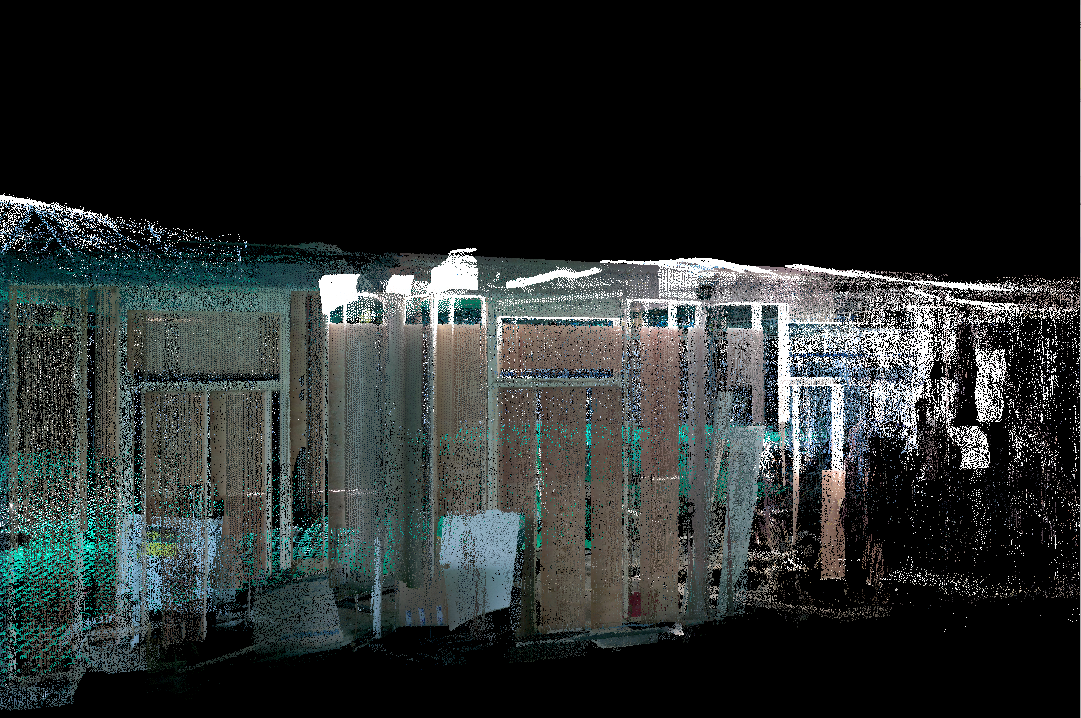
\includegraphics[width=.5\linewidth]{tuloksia/worksite_2M/worksite_overviewbuf.png}
    }
    \caption{Worksite-pilvi renderöity kahdella miljoonalla pisteellä käyttäen (a) pelkkää puskurivirtaa ja (b) yleiskuvapuskurin ja puskurivirran yhdistelmällä. Pistepilvi on Leica Geosystemsin omaisuutta.}
    \label{img:worksite_vertailu}
\end{figure}

Mittauksista selviää, että pelkän puskurivirran käyttäminen puun renderöinnissä on selkeästi nopeampaa kuin yleiskuvapuskurin ja puskurivirran yhdistelmällä. Tämä ero selittyy puun solmujen järjestämiseen vaaditulla ajalla. Vaikka järjestäminen vie arvokasta laskenta-aikaa, voidaan sen parantavan lopputuloksen laatua. Kuvassa \ref{img:worksite_vertailu} vasemmalla puolella näkyy, kuinka puskurivirta on renderöinyt koko näkyvillä olevan pistepilven samalla pistetiheydellä ja taaimmainen seinä näyttää tarkemmalta kuin kameraa lähempänä oleva. Oikeanpuoleisessa kuvassa puun solmut on yleiskuvan renderöinnin jälkeen järjestetty ruudulle projisoidun koon mukaan, minkä seurauksena etualalla oleva seinä näkyy selvästi. Solmujen järjestämistä voisi nopeuttaa helposti säikeistämällä renderöintialgortimi niin, että yksi säie valikoi puusta solmuja prioriteettijonoon, josta toinen säie ottaa aina suurimman prioriteetin omaavan solmun renderöitäväksi.

Kameran liikkuessa pistepilven ohi riittää usein renderöidä vain karkea yleiskuva pilvestä. Kun yleiskuvan pisteet pidetään näytönohjaimen muistissa, on niiden renderöiminen jokaisella ruudunpäivityksellä nopeaa. Kuvassa \ref{ws_ovw} on verrattu yleiskuvan renderöintiä kun yleiskuvapuskuri on valmiiksi näytönohjaimen muistissa siihen, kun pisteet ladataan keskusmuistista puskurivirralla näytönohjaimelle. Yleiskuvapuskurin tapauksessa renderöintiaika on mitattu piirtokomennon suorittamisesta siihen, että näytönohjain on saanut kaikki pisteet renderöityä ja merkattua synkronointiobjektin käsitellyksi. Näin kaikki pisteet on varmasti renderöity ruudulle ajastimen pysähtyessä. Pisteiden lataaminen levyltä ja kompression purkaminen on näissä mittauksissa jätetty pois.

\begin{figure}[h]
    \centering
    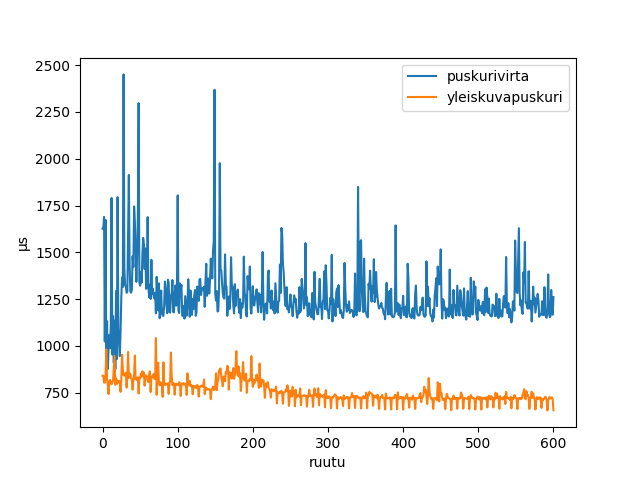
\includegraphics[width=0.9\textwidth]{tuloksia/worksite_overview.png}
    \caption{Worksite-pilvestä muodostetun puun viiden ylimmän tason renderöintiin käytetty aika mikrosekunteina puskurivirralla ja kun pisteet ovat valmiiksi yleiskuvapuskurissa näytönohjaimen muistissa.}
    \label{ws_ovw}
\end{figure}